\documentclass[14pt,a4paper,report]{report}
\usepackage[a4paper, mag=1000, left=2.5cm, right=1cm, top=2cm, bottom=2cm, headsep=0.7cm, footskip=1cm]{geometry}
\usepackage[utf8]{inputenc}
\usepackage[english,russian]{babel}
\usepackage{indentfirst}
\usepackage[dvipsnames]{xcolor}
\usepackage[colorlinks]{hyperref}
\usepackage{listings} 
\usepackage{fancyhdr}
\usepackage{caption}
\usepackage{amsmath}
\usepackage{graphicx}
\usepackage{amsmath}
\usepackage{booktabs}
\usepackage{array}
\newcolumntype{P}[1]{>{\centering\arraybackslash}p{#1}}
\hypersetup{
colorlinks = true,
linkcolor = black
}

\usepackage{titlesec}
\titleformat{\chapter}
{\Large\bfseries} % format
{} % label
{0pt} % sep
{\huge} % before-code


\DeclareCaptionFont{white}{\color{white}} 

% Listing description
\usepackage{listings} 
\DeclareCaptionFormat{listing}{\colorbox{gray}{\parbox{\textwidth}{#1#2#3}}}
\captionsetup[lstlisting]{format=listing,labelfont=white,textfont=white}
\lstset{ 
% Listing settings
inputencoding = utf8,	
extendedchars = \true, 
keepspaces = true, % Поддержка кириллицы и пробелов в комментариях
language = C, % Язык программирования (для подсветки)
basicstyle = \small\sffamily, % Размер и начертание шрифта для подсветки кода
numbers = left, % Где поставить нумерацию строк (слева\справа)
numberstyle = \tiny, % Размер шрифта для номеров строк
stepnumber = 1, % Размер шага между двумя номерами строк
numbersep = 5pt, % Как далеко отстоят номера строк от подсвечиваемого кода
backgroundcolor = \color{white}, % Цвет фона подсветки - используем \usepackage{color}
showspaces = false, % Показывать или нет пробелы специальными отступами
showstringspaces = false, % Показывать или нет пробелы в строках
showtabs = false, % Показывать или нет табуляцию в строках
frame = single, % Рисовать рамку вокруг кода
tabsize = 2, % Размер табуляции по умолчанию равен 2 пробелам
captionpos = t, % Позиция заголовка вверху [t] или внизу [b] 
breaklines = true, % Автоматически переносить строки (да\нет)
breakatwhitespace = false, % Переносить строки только если есть пробел
escapeinside = {\%*}{*)} % Если нужно добавить комментарии в коде
}

\begin{document}

\def\contentsname{Содержание}

% Titlepage
\begin{titlepage}
\begin{center}
\textsc{Санкт-Петербургский Политехнический 
Университет Петра Великого\\[5mm]
Кафедра компьютерных систем и программных технологий}

\vfill

\textbf{Отчёт по лабораторной работе №2\\[3mm]
Курс: «Интеллектуальные системы»\\[41mm]
}
\end{center}

\hfill
\begin{minipage}{.4\textwidth}
Выполнил студент:\\[2mm] 
Волкова М.Д.\\
Группа: 13541/2\\[5mm]

Проверил:\\[2mm] 
Болсуновская М.В.
\end{minipage}
\vfill
\begin{center}
Санкт-Петербург\\ \the\year\ г.
\end{center}
\end{titlepage}

% Contents
\tableofcontents
\clearpage

\chapter{Лабораторная работа №2}

\section{Цель работы}

Научиться оформлять отчеты по лабораторным работам.

\section{Программа работы}

\begin{enumerate}
\item Приведите интенсиональное и экстенсиональные определения двух понятий на ваш выбор.
\item Постройте ментальную модель знаний в предметной области по вашему выбору с помощью
интеллект-карт (http://www.mind-map.ru/), которая будет содержать не менее четырех уровней
ветвления.
\item Разработайте стратегию принятия решений о приеме на работу кандидата в выбранную Вами
компанию и записать решение в виде
\begin{enumerate}
\item набора продукционных правил (http://itteach.ru/predstavlenie-znaniy/produktsionnaya-model-predstavleniya-znaniy)
\item дерева принятия решений (http://logic.pdmi.ras.ru/~sergey/teaching/ml/notes-01-dectrees.pdf)
\item таблицы решений (http://5fan.ru/wievjob.php?id=14722)
\end{enumerate}
\item Выделите отличия и сходства следующих моделей представления знаний: алгоритмических,
логических, сетевых и продукционных и сценарий. Постарайтесь дать объяснения этим различиям.
\item Что такое онтологии, деревья, фреймы? В чем сходство и различие данных моделей?
\item Ознакомьтесь с теорией экспертных систем (ЭС). Опишите различие между базой данных (БД) и
базой знаний (БЗ). Что такое логика предикатов? Что такое «правило вывода»? В чем сильные и
слабые стороны любой ЭС?
\item Приведите не менее 3 примеров экспертных систем в каждой из предметных областей,
разработанную в последнее десятилетие (не позднее 2007), заполнить таблицу.
\end{enumerate}

\clearpage

\section{Ход работы}

\subsection{Задание 1}

\subsubsection{Приведите интенсиональное и экстенсиональные определения двух понятий на ваш выбор.}

\emph{\textbf{Ложка (интенсиональное)}} -- часть столового прибора, предмет, которым наливают или едят жидкости, накладывают или едят полужидкую, рассыпчатую пищу.

\emph{\textbf{Ложка (экстенсиональное)}} -- столовый прибор, такой как: половник, поварешка.

\emph{\textbf{Роликовые коньки (интенсиональное)}} -- ботинки с прикреплёнными к ним рамами, в которых закреплено от двух до пяти (и даже шести) колёс, предназначенные для передвижения по твёрдой ровной поверхности, реже по бездорожью, аналогично передвижению по льду на традиционных коньках. Используются как спортивный инвентарь, для занятий фитнесом и активного отдыха.

\emph{\textbf{Роликовые коньки (экстенсиональное)}} -- спортивный инвентарь для передвижения, такой как: скейт, велосипед, коньки.

\subsection{Задание 2}

\subsubsection{Постройте ментальную модель знаний в предметной области по вашему выбору с помощью интеллект-карт}

\begin{figure}[h!]
\centering
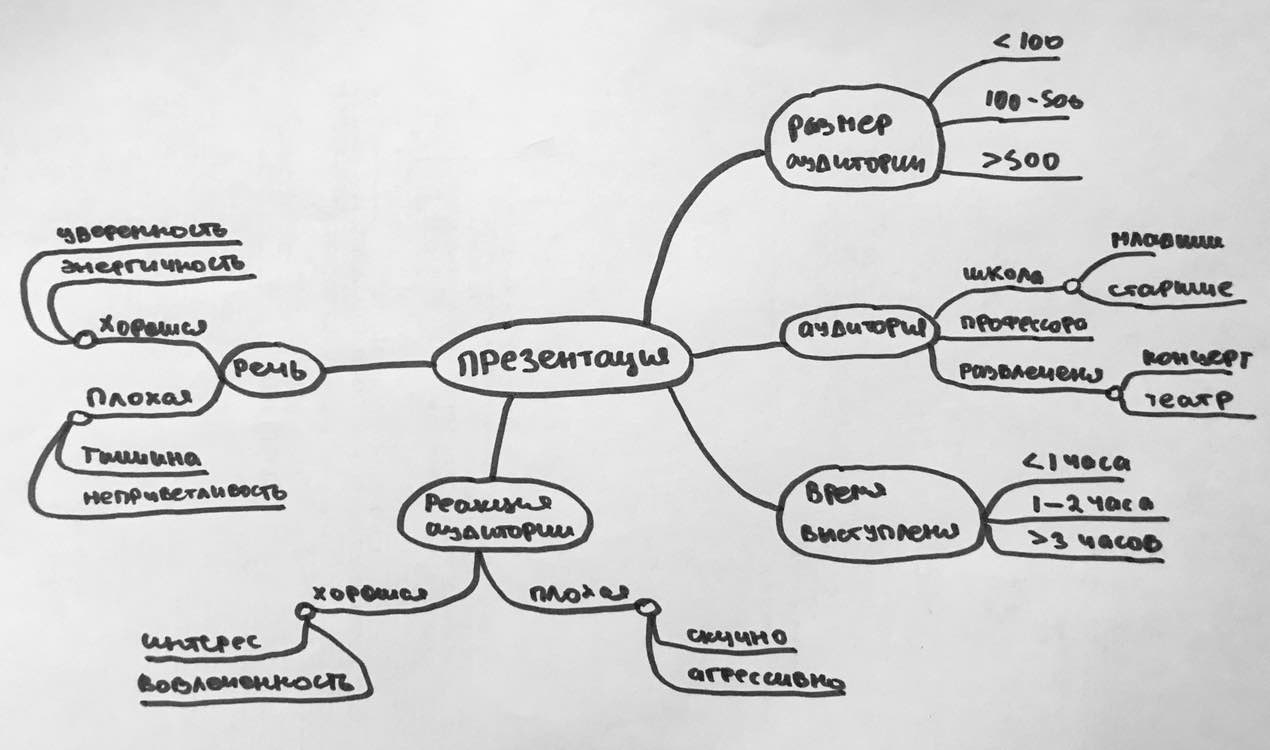
\includegraphics[scale = 0.35]{images/mindmap.jpg}
\caption{Ментальная модель знаний}
\label{image:1}
\end{figure}

\subsection{Задание 3}

Кандидат: успешно прошел собеседование

\subsubsection{Стратегия принятия решений о приеме на работу кандидата в виде набора продукционных правил}


П1: Если (кандидат - имеет высшее образование) то (кандидат - подходит).

П2: Если (кандидат - успешно прошел собеседование) то (кандидат - подходит).

П3: Если (кандидат - подходит) то (работа - принять на работу).

\textbf{1-ый проход}

Шаг 1. П1: не работает (не хватает данных (кандидат - имеет высшее образование)).

Шаг 2. П2: работает, в базу поступает факт (кандидат - подходит).

Шаг 3. П3: работает, в базу поступает факт (работа - принять на работу).

\textbf{Вывод: принять на работу}

\subsubsection{Стратегия принятия решений о приеме на работу кандидата в виде дерева принятия решений}

\begin{figure}[h!]
\centering
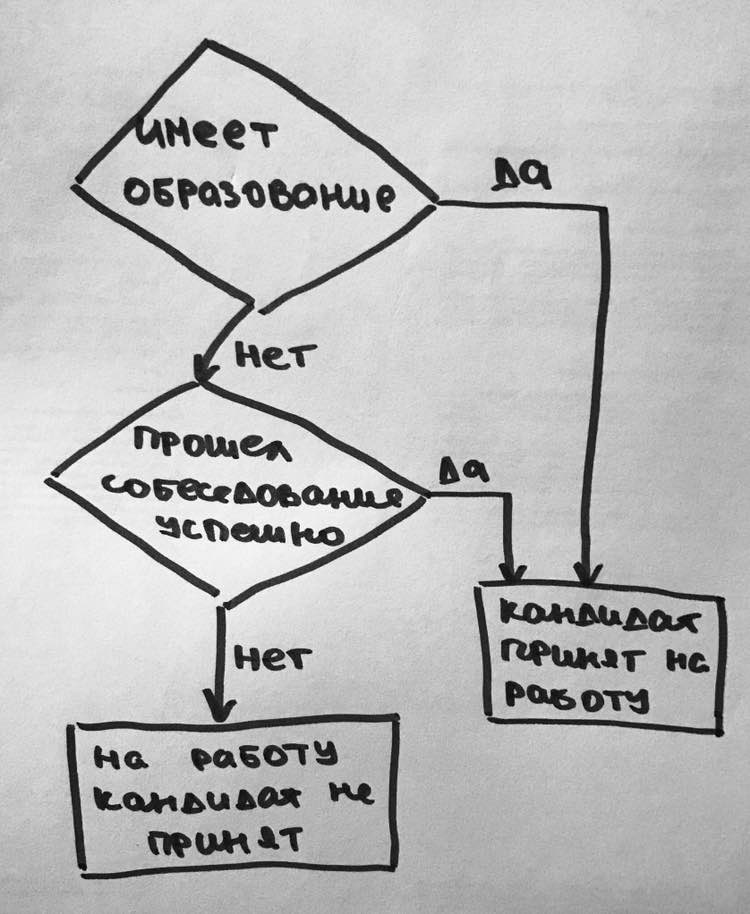
\includegraphics[scale = 0.40]{images/tree.jpg}
\caption{Дерево принятия решений}
\label{image:2}
\end{figure}

\clearpage

\subsubsection{Стратегия принятия решений о приеме на работу кандидата в виде таблицы решений}

\begin{table}[h!]
\centering
\bgroup
\def\arraystretch{1}
\begin{tabular}{ | c| c | c | }
\hline
имеет высшее образование & успешно прошел собеседование & результат 
\\ \hline

- & - & - \\ \hline

- & + & + \\ \hline

+ & - & + \\ \hline

+ & + & + \\ \hline


\end{tabular}
\egroup
\caption{Таблица решений}
\label{table:1}
\end{table}

\subsection{Задание 4}

\subsubsection{Выделите отличия и сходства следующих моделей представления знаний: алгоритмических, логических, сетевых и продукционных и сценарий. Постарайтесь дать объяснения этим различиям.}

Алгоритмические модели - это те, в которых критерии описываются математическими конструккциями. Логические - описывается совокупностью фактов и утверждений, которые представляются в виде некоторой логики. Сетевые - показывают взаимосвязи между операциями, строго распределенных по времени. Продукционные - модели, основанные на правилах, позволяющих представить знание в виде предложений типа: «ЕСЛИ (условие), ТО (действие)» 

Один и тот же процесс можно представить несколькими моделями. 

\subsection{Задание 5}

\subsubsection{Что такое онтологии, деревья, фреймы? В чем сходство и различие данных моделей?}

\textbf{Онтология} -- это формальное описание результатов концептуального моделирования предметной области, представленная в форме, воспринимаемой человеком и компьютерной системой [1]

\textbf{Дерево принятия решений} -- дерево, в листьях которого стоят значения целевой функции, а в остальных узлах -- условия перехода, определяющие по какому из ребер идти [2]

\textbf{Фрейм} -- структура данных для представления некоторого концептуального объекта. Информация, относящаяся к фрейму, содержится в составляющих его слотах. Каждый фрейм состоит из произвольного числа слотов, причем несколько из них обычно определяются самой системой для выполнения специфических функций, а остальные определяются пользователем. [3]

Дерево легче описывается алгоритмами, онтология более показательная, а фреймы исспользуются, когда большое количество парамметров.

\subsection{Задание 6}

\subsubsection{Ознакомьтесь с теорией экспертных систем (ЭС). Опишите различие между базой данных (БД) и базой знаний (БЗ). Что такое логика предикатов? Что такое правило вывода? В чем сильные и слабые стороны любой ЭС?}

База знаний -- это семантическая модель, описывающая предметную область и позволяющая отвечать на такие вопросы из этой предметной области, ответы на которые в явном виде не присутствуют в базе. А в базе данных хранятся материалы, связанные между собой. 

\textbf{Логика предикатов} -– раздел современной логики символической, изучающий рассуждения и другие языковые контексты с учетом внутренней структуры входящих в них простых высказываний, при этом выражения языка трактуются функционально, т.е. как знаки некоторых функций или же знаки аргументов этих функций [4]

\textbf{Правило вывода} -- если известно, что высказывание «А» влечет (имплицирует) высказывание «В», а также известно, что высказывание «А» истинно, то, следовательно, «В» истинно [5]

Трудно говорить о сильных сторонах экспертных систем в настоящее время. А вот из слабых: они неспособны к самообучению. Для того, чтобы поддерживать экспертные системы в актуальном состоянии необходимо постоянное вмешательство в базу знаний инженеров по знаниям. Экспертные системы, лишенные поддержки со стороны разработчиков, быстро теряют свою востребованность.


\clearpage

\subsection{Задание 7}

\subsubsection{Приведите не менее 3 примеров экспертных систем в каждой из предметных областей, разработанную в последнее десятилетие (не позднее 2007), заполнить таблицу.}

\begin{table}[h!]
\centering
\bgroup
\def\arraystretch{1}
\begin{tabular}{ | P{2cm} | P{13cm} | P{1cm} | P{0.5cm} | }
\hline
Предметная область & Название, Страна, Краткое описание & Год & Ссылка 
\\ \hline

Геология 

& \textbf{HASP/SIAP} (Россия) -- интерпретирующая система, которая определяет местоположение и типы судов в Тихом океане по данным акустических систем слежения. & 2009 & [6] \\ \hline

& \textbf{ASTA} (Россия) -- Экспертная система помогает аналитику определить тип радара, пославшего перехваченный сигнал. Система анализирует этот сигнал в свете имеющихся у нее общих знаний о физике радаров и специальных знаний о конкретных типах радарных систем. ASTA также помогает аналитику, обеспечивая ему доступ к соответствующим базам данных и давая объяснения своим заключениям. Знания в системе представлены в виде правил. & 2015 & [7] \\ \hline

& \textbf{PROSPECTOR} (США) -- действует как консультант, помогающий геологам в поисках залежей руд. Получив данные о геологии района, система оценивает вероятность обнаружить в нем определенные виды минеральных отложений. & 1977 & [8] \\ \hline


Юриспруденция 

& \textbf{SAL} (Россия) -- поддерживает юристов при установлении размеров исков, связанных с профессиональными заболеваниями работников, которые работают с асбестом. & 2007 & [9] \\ \hline

& \textbf{TAXMAN} (Россия) -- помогает исследовать логику рассуждений и аргументацию на примере законодательства о налогообложении корпораций. & 2012 & [10] \\ \hline

& \textbf{LDS} (США) -- помогает юристам урегулировать проблемы исков о возмещении убытков и компенсациях за ущерб, связанный с выпуском дефектной продукции. Система на основе описания дела выдвигает версию о виновности ответчика, определяет цену иска, размер компенсации, который обеспечивает интересы сторон. & 1993 & [11] \\ \hline


Медицина 

& \textbf{simptomus} (Россия) -- поиск заболеваний по симптомам & 2011 & [12] \\ \hline

& \textbf{MYCIN} (Великобритания) -- наиболее известная диагностическая система, которая предназначена для диагностики и наблюдения за состоянием больного при менингите и бактериальных инфекциях. & 2009 & [13] \\ \hline

& \textbf{Кардиолог} (Россия) -- определяет диагноз больного по введенным симптомам, назначает курс лечения и профилактики. & 2011 & [14] \\ \hline


Экономика 

& \textbf{IW} (Великобритания) -- Экспертная система помогает аналитикам из разведки предсказывать, когда и где произойдет следующее вооруженное столкновение. Система анализирует поступающие сообщения разведки, например донесения о местонахождении воинских соединений, их деятельности и передвижениях, применяя знания об обычных признаках активности войск. Знания представлены в рамках архитектуры доски объявлений, в которой для обеспечения компетентности применены как правила с прямой цепочкой рассуждений, так и фреймы. Система реализована на языке INTERLISP-D для АРМ Xerox 1100. Она разработана компанией ESL в сотрудничестве со Стенфордским университетом и доведена до уровня демонстрационного прототипа. & 2014 & [15] \\ \hline

& \textbf{SPCBRS } (США) -- Разработчиком данной экспертной системы является Chase Manatten Bank, Standart Poor's Corp. SPCBRS была разработана для решения следующих задач: оценка рейтинга ценных бумаг по данным о фирмах эмитентах; формирование корректной рейтинговой шкалы. Экспертная система имеет следующие характеристики: представление задачи оценки рейтинга как задачи классификации; отбор данных о фирмах эмитентах и формирование обучающего материала; выбор нейроклассификатора, его обучение и тестирование; сравнение с оценками экспертов; использование нейросетевой парадигмы Couter-Propagation.Вероятность правильного предсказания рейтинга экспертной системы SPCBRS составляет 84 процента. & 2009 & [16] \\ \hline

& \textbf{G2 Expert System} (США) -- автоматизация принятия решений при больших рисках. & 2009 & [17] \\ \hline


Биология 

& \textbf{DENDRAL} (США) -- это старейшая, самая разработанная экспертная система, определяющая строение органических молекул по химическим формулам и спектрографическим данным о химических связях в молекулах. Была создана в Стэнфорде. & 2008 & [18] \\ \hline

& \textbf{CASSIOPE} (США) -- помогает специалистам по структурной химии определять наборы возможных структур неизвестных соединений. & 2009 & [19] \\ \hline

& \textbf{Мolgen Five} (Германия) -- экспертная системя для генеалогического тестирования. & 2008 & [20] \\ \hline

\end{tabular}
\egroup
\caption{Примеры экспертных систем}
\label{table:2}
\end{table}

\section{Вывод}

В этой лабораторной работе мы изучили понятие экспертных систем. Было выявленно, что в настоящее время концепция экспертных систем, переживает серьёзный кризис, связанный с её глубокой ориентацией на текстовый человеко-машинный интерфейс, который в настоящее время вытеснен графическим интерфейсом. Кроме того, «классический» подход к построению экспертных систем плохо согласуется с реляционной моделью данных, что делает невозможным эффективное использование современных промышленных СУБД для организации баз знаний таких систем.

\clearpage

\section{Список литературы}


\begin{flushleft}

[1] Онтология [Электронный ресурс]. — URL: http://www.aiportal.ru/articles/other/ontology.html

[2] Классификация и регрессия с помощью деревьев принятия решений [Электронный ресурс]. — URL: https://habrahabr.ru/post/116385/

[3] Технология баз информации. Информационное обеспечение процессов управления в экономике [Электронный ресурс]. — URL: https://www.intuit.ru/studies/courses/3735/977/lecture/14681?page=4

[4] ЛОГИКА ПРЕДИКАТОВ [Электронный ресурс]. — URL: https://iphlib.ru/greenstone3/library/collection/newphilenc/document/HASHb46c37179b4005520488b4

[5] Правила вывода [Электронный ресурс]. — URL: http://www.aiportal.ru/articles/knowledge-models/modus-ponens.html

[6] HASP/SIAP [Электронный ресурс]. — URL: https://stacks.stanford.edu/file/druid:gv051pd9022/gv051pd9022.pdf
[7] ASTA [Электронный ресурс]. — URL: https://www.intuit.ru/studies/courses/651/507/lecture/11533
[8] PROSPECTOR [Электронный ресурс]. — URL: https://habr.com/post/247221/

[9] Sal [Электронный ресурс]. — URL: http://lybs.ru/index-841.htm
[10] TAXMAN [Электронный ресурс]. — URL: https://www.law.georgetown.edu/experiential-learning/centers-institutes/
[11] LDS [Электронный ресурс]. — URL: http://lybs.ru/index-841.htm

[12] simptomus [Электронный ресурс]. — URL: http://simptomus.ru
[13] MYCIN [Электронный ресурс]. — URL: http://www.cs.utexas.edu/users/novak/tmycin.html
[14] Кардиолог [Электронный ресурс]. — URL: https://bourabai.ru/alg/expert21.htm

[15] IW [Электронный ресурс]. — URL: http://www.aiportal.ru/articles/expert-systems/examples-expsys.html
[16] SPCBRS [Электронный ресурс]. — URL: https://bourabai.ru/alg/expert21.htm
[17] Nereid [Электронный ресурс]. — URL: https://bourabai.ru/alg/expert21.htm

[18] DENDRAL [Электронный ресурс]. — URL: https://ruslion.ru/psyhology/psychology76.html
[19] CASSIOPE [Электронный ресурс]. — URL: http://dspace.nbuv.gov.ua/xmlui/bitstream/handle/123456789/60482/59-Ruchkin.pdf?sequence=1
[20] Мolgen Five [Электронный ресурс]. — URL: https://books.ifmo.ru/file/pdf/1080.pdf


\end{flushleft}



\end{document}